\chapter{Introducción a la Programación Concurrente}
\section{Conceptos básicos}
Hasta ahora, nos hemos dedicado al estudio y desarrollo de programas secuenciales, que podemos entender de forma intuitiva como una ejecución lineal de instrucciones.\\

En programación concurrente, tendremos ahora múltiples unidades de ejecución independientes, a las que llamaremos procesos (sea un core o un procesador). La programación concurrente trata de coordinar los procesos para que cooperen entre sí con el fin de realizar un problema global de forma mucho más rápida de como lo haría un programa secuencial.\\

Podemos pensar que un proceso es una unidad de software abstracta conformada por con un conjunto de instrucciones a ejecutar y por el contexto del procesador (como los valores de los registros, el contador de programa, el puntero de pila, la memoria Heap, memoria para variables, el acceso a determinados recursos, \ldots), al que llamamos estado del proceso.\\

Cuando en esta asignatura aparezca ``flujo de control'', debemos pensar en una secuencia de ejecución de instrucciones. Es decir, como si fuera un proceso pero carente de un estado.\\

Nuestro trabajo en esta asignatura será gestionar la concurrencia, es decir, la ejecución independiente de dichos procesos con el fin de que no sea una sucesión de eventos incontrolados.

% // TODO: Cambiar este titulo
\subsection{Comparación de programas concurrentes con secuenciales}
Normalmente, en un programa concurrente tendremos más procesos que núcleos donde ejecutar dichos procesos, de donde aparece el concepto de concurrencia: en programación concurrente debe parecer que todos los procesos avanzan de forma simultánea, pese a haber más procesos que núcleos.\\

Si provocamos cambios de contexto dejando avanzar al resto de flujos de control, el programa no sufrirá las latencias provocadas por los procesos de E/S (por ejemplo), haciendo que el programa global sea más eficiente gracias a la concurrencia.\\

En sistemas que simulen el mundo real, podemos asociar un proceso con cada ente que intervenga en nuestro sistema (como una simulación del tráfico en una ciudad, o del movimiento de planetas), con lo que los sistemas de simulación pueden modelarse mejor con procesos concurrentes independientes, más que con programas secuenciales.

\subsection{Definición de concurrencia}
Podríamos definir la concurrencia como el paralelismo potencial que existe en los programas que puede aprovecharse independientemente de las limitaciones del hardware en el que se ejecuta el programa.\\

Como ya hemos mencionado, podremos tener un mayor número de procesos que de cores, y con este modelo cada uno de los procesos se ejecuta aparentemente al mismo tiempo que los demás.\\

El concepto de concurrencia es un concepto de programación a alto nivel que trata de representar el paralelismo potencial que existe en un programa. Con los compiladores adecuados, podemos programar en función de dichas características sin limitarnos por la arquitectura hardware del ordenador.\\

El objetivo fundamental de la concurrencia es simplificar toda la parte de la sincronización y comunicación entre los diferentes procesos de un programa, el cual suele ser un problema complejo sin solución fácil. Nos da un nivel algorítmico suficientemente independiente de los detalles del hardware para resolver dichos problemas, facilitando la portabilidad del código entre arquitecturas y lenguajes de programación.\\

\noindent
Como beneficios de este modelo abstracto (el de la concurrencia), podemos destacar:
\begin{itemize}
    \item Da herramientas, instrucciones y sentencias útiles para problemas de sincronización entre procesos.
    \item Las primitivas de programación en un lenguaje de alto nivel (como son los lenguajes concurrentes) son más fáciles de utilizar que con lenguajes de bajo nivel. Por ejemplo, los semáforos son más complejos que los monitores.
    \item Evita la dependencia con instrucciones de bajo nivel, haciendo que el programa pueda ejecutarse en otra computadora.
\end{itemize}

\subsection{Axiomas de la programación concurrente}
La programación concurrente es un modelo abstracto definido en base a 5 axiomas que nos dicen si un lenguaje es o no concurrente. En caso de no cumplirse, el código no va a poder ser transportable ni verificable.

Estos axiomas son:
\begin{description}
    \item [1. Atomicidad y entrelazamiento de instrucciones atómicas.]~\\
        Al menos ciertas instrucciones han de ser atómicas (esto es, instrucciones que no pueden ser interrumpidas, como por ejemplo las lecturas y escrituras en memoria).
    \item [2. Consistencia de los datos tras un acceso concurrente.]~\\
        El entrelazamiento de instrucciones atómicas preserva la
        consistencia de los resultados de las operaciones. 
        Es decir, si tenemos muchos procesos actuando a la vez sobre un conjunto de datos compartidos, debemos estar seguros de que los accesos a los mismos no los estropeen.
    \item [3. Irrepetibilidad de las secuencias de instrucciones.]~\\
        Cuando se ejecuta un programa concurrente, se sucede un entrelazamiento de las instrucciones de los procesos que se ejecutan a la vez, con lo que la secuencia de instrucciones que obtenemos como resultado de volver a ejecutar el mismo programa con otros datos es muy probable que no sea la misma.

        Esto dificulta el ``debugging'' de un programa concurrente, ya que podemos tener un error en el programa que repercuta en el mal funcionamiento del mismo sólo cuando se suceda una secuencia de instrucciones específica en la ejecución del mismo.
    \item [4. Independencia de la velocidad de los procesos.]~\\
        No puede hacerse ninguna suposición en la velocidad de ejecución de un proceso, ya que este puede verse suspendido o ralentizado, salvo que esta es positiva.

        La corrección en programas concurrentes no debe depender de la velocidad relativa de los procesos.
    \item [5. Hipótesis del progreso finito.]~\\
        \begin{itemize}
            \item Un proceso debe tratar de avanzar todo lo que pueda. Esto es, si un proceso se está ejecutando, debe tratar de ejecutar tantas instrucciones como sea posible.
            \item Una vez que un proceso comienza a ejecutar una sección de código, debe terminar dicha sección.
            \item Todo proceso debe seguir progresando durante la ejecución de un programa.
        \end{itemize}
\end{description}

\noindent
Cuando se interpreta la ejecución de un programa concurrente como un conjunto de trazas de las cuales elegimos una al ejecutar el programa, estamos ignorando ciertos detalles, como:
\begin{itemize}
    \item El estado de la memoria asignado a cada proceso.
    \item El valor de los registros de cada proceso.
    \item El coste computacional de los cambios de contexto.
    \item La política de planificación que se emplea de los procesos.
    \item El desarrollo de los programas es independiente del hardware.
\end{itemize}

\section{Modelos para creación de procesos en un programa}
En relación al número de procesos que se ejecutan en un programa, podemos clasificarlos en:
\begin{itemize}
    \item Sistemas estáticos: El número de procesos en el programa es el mismo durante su ejecución. Dicho número se define al programarlo y en el momento de la compilación.
    \item Sistemas dinámicos: El número de procesos es variable, de forma que durante la ejecución del programa pueden crearse y destruirse procesos.
\end{itemize}

\subsection{Grafos de Sincronización}
Un Grafo de Sincronización es un Grafo Dirigido Acíclico (DAG) donde cada nodo representa una secuencia de sentencias del programa (o actividad). Nos sirven para definir situaciones de precedencia en la ejecución de un programa. Tenemos que tener instrucciones en el lenguaje concurrente que nos permitan representar el comienzo de las instrucciones con un DAG\@.\\

En un DAG, se suceden dependencias secuenciales, esto es, un proceso no empieza hasta que termina otro: dadas dos actividades $S_1$ y $S_2$, una arista desde la primera hacia la segunda ($S_1\rightarrow S_2$) significa que $S_2$ no puede comenzar su ejecución hasta que $S_1$ haya finalizado.\\

\begin{ejemplo}
    El DAG de la Figura~\ref{fig:primer_dag} nos indica que la primera actividad que tendrá lugar en nuestro programa será la actividad $S_1$. Tras el fin de esta, se sucederán de forma concurrente las actividades $S_2$ y $S_3$. Tras terminar $S_2$, comenzará $S_4$ y, tras esta, se ejecutarán de forma concurrente $S_5$ y $S_6$. Finalmente, tras el final de $S_5$, $S_6$ y $S_3$, el programa terminará con la actividad $S_7$.

    \begin{figure}[H]
    \centering
    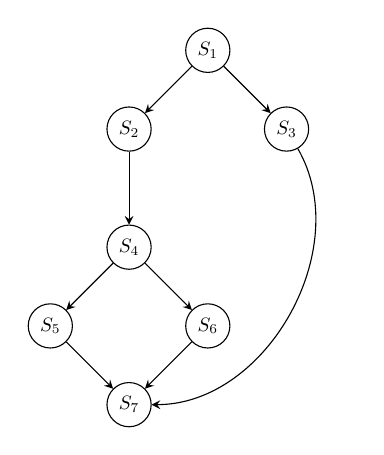
\begin{tikzpicture}
        \node[draw, circle, scale=0.7] (A) at (0,0) {$S_1$};
        \node[draw, circle, scale=0.7] (B) at (-1,-1) {$S_2$};
        \node[draw, circle, scale=0.7] (C) at (1,-1) {$S_3$};
        \node[draw, circle, scale=0.7] (D) at (-1,-2.5) {$S_4$};
        \node[draw, circle, scale=0.7] (E) at (-2,-3.5) {$S_5$};
        \node[draw, circle, scale=0.7] (F) at (0,-3.5) {$S_6$};
        \node[draw, circle, scale=0.7] (G) at (-1,-4.5) {$S_7$};
        
        \draw[-stealth] (A) -- (B);
        \draw[-stealth] (A) -- (C);
        \draw[-stealth] (B) -- (D);
        \draw[-stealth] (D) -- (E);
        \draw[-stealth] (D) -- (F);
        \draw[-stealth] (E) -- (G);
        \draw[-stealth] (F) -- (G);

        \draw[-stealth] (C) to[out=300, in=0] (G);
    \end{tikzpicture}
    \caption{Ejemplo de DAG}
    \label{fig:primer_dag}
    \end{figure}
\end{ejemplo}

\noindent
En relación a cómo podemos crear los procesos, destacamos dos formas que podemos encontrarnos en los lenguajes paralelos:

\subsection{Definición estructurada de procesos}
En programación estructurada, contaremos con dos palabras reservadas del lenguaje que nos permitirán recrear la siguiente funcionalidad a explicar. En pseudocódigo, nos referiremos a ellas como \verb|cobegin| y \verb|coend|.\\

Dados dos procesos $P_1$ y $P_2$ que queremos que se ejecuten de forma concurrente, bastará especificar en pseudocódigo:
\begin{minted}{pascal}
    cobegin
      P1; 
      P2; 
    coend
\end{minted}
Hasta llegar a la palabra \verb|cobegin| no comenzará ningún proceso. Tras esta, se sucederá un entrelazado de las instrucciones de $P_1$ y $P_2$, y no se saldrá de dicha región hasta que terminen ambos procesos.

\begin{ejemplo}
    Un programa utilizando la definición estructurada de procesos que cumpla el DAG de la Figura~\ref{fig:primer_dag} es el siguiente:
    \begin{minted}{pascal}
    begin
      S1;
      cobegin
        begin
          S2;
          S4;
          cobegin
            S5;
            S6;
          coend
        end
        S3;
      coend
      S7;
    end
    \end{minted}
\end{ejemplo}

\subsection{Definición no estructurada de procesos}
En lenguajes concurrentes que no cuenten con palabras reservadas que simulen \verb|cobegin| y \verb|coend|, contaremos con dos llamadas al sistema que nos permitirán replicar dicha funcionalidad para crear procesos:
\begin{description}
    \item [fork]~\\
        Duplica el proceso que actualmente se está ejecutando y lo lanza a ejecución. Si se le especifica una rutina, cambiará el código del clon por dicha rutina.
    \item [join]~\\
        Espera a que cierto proceso termine de ejecutarse antes de proseguir con la ejecución del resto de instrucciones.
\end{description}
La función \verb|fork| ya se vió en la asignatura de Sistemas Operativos, por lo que el estudiante debería estar familiarizado con ella.

\begin{ejemplo}
    Un programa con definición no estructurada de procesos para el DAG de la Figura~\ref{fig:primer_dag} es el siguiente:
    \begin{minted}{pascal}
    begin        
      S1;
      fork S3;
      S2;
      S4;
      fork S6;
      S5;
      join S3;
      join S6;
      S7;
    end
    \end{minted}
\end{ejemplo}

\section{Exclusión mutua y sincronización}
No todas las secuencias de entrelazamiento de un programa concurrente van a ser aceptables. Para impedir que sucedan ciertas secuencias (o trazas) tenemos condiciones de sincronización, relacionadas con instrucciones de lenguajes de programación de tal forma que dichas instrucciones no se ejecutan hasta que no es cierta una condición que depende de las variables del proceso.

De esta forma, una \textbf{condición de sincronización} es una restricción en el orden en que se pueden entremezclar las instrucciones que generan los procesos de un programa. Podemos utilizarlas para asegurarnos de que todas las trazas del programa son correctas.\\

La \textbf{exclusión mutua} es un caso particular de sincronización en el que se obliga a que un trozo de código de un proceso sea ejecutado de forma totalmente secuencial de manera que no se permita el entrelazamiento con otros procesos. Este trozo de código (en el que no se permite el entrelazamiento de instrucciones con otros procesos) recibe el nombre de \textbf{sección crítica}. Se dice que las secciones críticas se ejecutan en exclusión mutua.\\

La mayoría de instrucciones en un programa son instrucciones compuestas (esto es, formadas por varias instrucciones en lenguaje máquina). Si queremos establecer secciones críticas para la ejecución de cada una de dichas instrucciones, rodearemos la instrucción por \verb|<| y \verb|>|.
Notaremos así que se ejecuta de forma atómica.

\begin{ejemplo}
    Por ejemplo, ante el siguiente código concurrente:
    \begin{minted}{pascal}
    begin
      x := 0;
      cobegin
        x := x+1;
        x := x-1;
      coend
    end
    \end{minted}
    El resultado obtenido en la variable \verb|x| es indeterminado, ya que puede ser $1$, $-1$ o $0$:
    \begin{itemize}
        \item El segundo proceso puede leer la variable \verb|x| antes de que el primero escriba en ella, leyendo 0; y podría escribir en ella después de que lo haga el primer proceso, escribiendo finalmente un $-1$.
        \item Podría ejecutarse el primer proceso antes que el segundo, dejando la variable \verb|x| a 1 y el segundo le cambiaría el valor a 0.
        \item El primer proceso puede leer la variable \verb|x| antes de que el segundo escriba en ella, leyendo 0; y podría escribir en ella después de que lo haga el segundo proceso, escribiendo finalmente un 1.
    \end{itemize}
    Notemos que esto sucede ya que la instrucción \verb|x := x OP a| es una instrucción compuesta de las instrucciones máquina: \verb|LOAD x|, \verb|OP a, x| y \verb|STORE x|.

    Sin embargo, ante el siguiente código concurrente:
    \begin{minted}{pascal}
    begin
      x := 0;
      cobegin
        < x := x+1 >;
        < x := x-1 >;
      coend
    end
    \end{minted}
    Obtenemos siempre 0 en \verb|x|, ya que las instrucciones de cada instrucción compuesta no se entrelazan, al ser secciones críticas. 
\end{ejemplo}

\subsubsection{Paradigma del Productor Consumidor}
El paradigma del productor/consumidor es una situación de dos procesos que cooperan, uno escribiendo datos en una variable, al que llamaremos productor; y otro que leerá dicha variable y realizará cálculos con ella, al que llamaremos consumidor.

Este paradigma nos sirve de ejemplo para justificar las condiciones de sincronización, así como para ponerlas en práctica.\\

Son necesarias condiciones de sincronización ya que no todas las trazas de ejecución de un programa con estructura productor/consumidor son correctas.

\begin{ejemplo}
    Si notamos por $L$ a las lecturas del consumidor y por $E$ a las escrituras del productor, las tres siguientes trazas de ejecución no son correctas:
    \begin{enumerate}
        \item \verb|L, E, L, E, ...|, porque leemos una lectura de la variable antes de que el productor escriba en ella, leyendo un valor indeterminado y pudiendo provocar el fallo del programa.
        \item \verb|E, L, E, E, L, ...|, porque el consumidor se ha perdido una escritura del productor en la variable, que puede hacer que cambie la salida del programa a una errónea.
        \item \verb|E, L, L, E, L, ...|, porque el consumidor ha usado un mismo dato dos veces, que también puede resultar en un mal funcionamiento del programa.
    \end{enumerate}
\end{ejemplo}

Para que el paradigma del productor/consumidor funcione correctamente, han de cumplirse las dos condiciones de sincronización siguientes:
\begin{enumerate}
    \item El consumidor no puede leer la variable hasta que el productor haya escrito en ella. Cuando el consumidor lee, debe esperar a que el productor proporcione un nuevo dato antes de volver a leer.
    \item El productor no puede escribir un nuevo valor hasta que el consumidor haya leido el último dato escrito (salvo en el primer valor a escribir).
\end{enumerate}
Para cumplir con las condiciones de sincronización, deberemos añadir instrucciones en el código para que:
\begin{itemize}
    \item El consumidor se detenga la primera vez hasta que el productor escriba en la variable.
    \item Se impida un segundo ciclo del consumidor hasta que se produzca el siguiente dato.
    \item Se impida un segundo ciclo del productor hasta que el dato anterior no haya sido leído por el consumidor.
\end{itemize}

\section{Propiedades de los sistemas concurrentes}
Una propiedad de un sistema concurrente es un atributo que se cumple en toda la ejecución del sistema, mientras que el conjunto de todas sus ejecuciones (de todas las posibles trazas generadas en la ejecución) nos dan el comportamiento del sistema.

Cualquier propiedad de un sistema concurrente puede ser formulada como combinación de dos tipos de propiedades fundamentales:

\begin{itemize}
    \item Propiedades de seguridad (\textit{safety}): Una propiedad de este tipo afirma que hay un estado del programa que es inalcanzable.
    \item Propiedades de vivacidad (\textit{liveness}): Propiedades que afirman que en algún momento se alcanzará un estado deseado.
\end{itemize}

\subsection{Propiedades de seguridad (\textit{safety})}
Estas propiedades expresan determinadas condiciones que han de cumplirse durante toda la ejecución del programa. Cualquier propiedad que pueda ser formulada por la existencia de un estado inalcanzable, es una propiedad de seguridad. En dicho caso, deberíamos poder definir qué estado es inalcanzable y demostrar que el programa concurrente nunca puede llegar a dicho estado.

Las propiedades de seguridad pueden ya comprobarse en tiempo de compilación, ya que se cumplen independientemente de la ejecución concreta que sigue el sistema en tiempo de ejecución. Es por esto que se trata de una propiedad estática.\\

Ejemplos de problemas donde vemos propiedades de seguridad son:
\begin{itemize}
    \item El problema de la exclusión mutua: La condición de que dos procesos del programa no puedan ejecutar simultáneamente las instrucciones de una sección crítica es de seguridad.
    \item Problema del productor/consumidor: Todos los estados que lleven a una traza distinta de \verb|E, L, E, L,| \ldots son estados prohibidos.
    \item La situación de interbloqueo: Es una de las situaciones más críticas que se dan tras quebrantar una propiedad de seguridad, ya que hay procesos ocupando recursos que no están usando y que no liberarán.
\end{itemize}

\subsection{Propiedades de vivacidad (\textit{liveness})}
Las propiedades de vivacidad expresan que el sistema llegará en un futuro a cumplir determinadas condiciones (en un tiempo no indeterminado). En determinados ejemplos, dichas propiedades pueden entenderse como que las condiciones dinámicas de ejecución no lleven a que determinados procesos sean sistemáticamente adelantados por otros, no pudiendo avanzar en la ejecución de instrucciones útiles, de forma que el proceso sufra inanición (\textit{starvation}).

Para demostrar que una propiedad es de vivacidad, debemos definir un ``buen estado'' del programa, y demostrar que es alcanzable para todos los procesos en un determinado tiempo.\\

Ejemplos de problemas donde vemos propiedades de vivacidad son:
\begin{itemize}
    \item El problema de la exclusión mutua: Las secciones críticas se ejecutan por un proceso a vez. El sistema debe garantizar que, en la espera por entrar a una región crítica, no ocurra que un proceso sea siempre adelantado por otros procesos, llevando a que dicho proceso nunca ejecute la región crítica (que es nuestro estado deseado).
    \item El problema del productor/consumidor: Un proceso que quiera escribir o leer de la variable compartida ha de poder hacerlo en un tiempo finito.
\end{itemize}

Debemos notar que el axioma de progeso finito expuesto en secciones anteriores no tiene nada que ver con la ausencia de inanición:
\begin{itemize}
    \item El axioma de progeso finito afirma que los procesos no pueden quedarse parados arbitrariamente, sino que estos deben intentar ejecutar instrucciones conforme les sea posible.
    \item Un proceso puede estar ejecutando instrucciones en un bucle indefinido pero no avanzar en la ejecución de las instrucciones de su código (es decir, puede estar realizando un trabajo inútil). En este caso, se cumpliría el axioma del progeso finito pero no se cumpliría la propiedad de vivacidad, ya que el proceso sufriría inanición.
\end{itemize}

Como ya venimos avisando, el no cumplimiento de la propiedad de vivacidad puede llevar a uno o más procesos a un estado de inanición (es indefinidamente pospuesto por otros, de forma que no pueda realizar aquello para lo que está programado). Aunque dicha situación es menos grave que una situación de interbloqueo (ya que hace que el programa no avance nada), tenemos procesos inoperantes (que no realizan su trabajo), por lo que consideraríamos que el programa concurrente no es correcto.\\

De esta forma, un programa concurrente solo podrá ser completamente correcto cuando se demuestre que los procesos que lo integran no sufren inanición en ninguna de sus posibles ejecuciones.

\begin{ejemplo}[Cena de filósofos]
    Disponemos de cinco filósofos, $F_0$, $F_1$, $F_2$, $F_3$ y $F_4$, que dedican su vida a pensar y en algún momento desean comer. Acceden a una mesa redonda en la que hay un plato del que todos pueden comer, siempre y cuando dispongan de dos palillos. Sólo hay 5 palillos, estos distribuidos de forma que entre dos filósofos hay un palillo.

    Los filósofos son cabezotas, por lo que una vez congen un palillo, no están dispuestos a soltarlo. Además, no pueden arrebatar un palillo a otro filósofo por ir en contra de sus ideales morales.\\

    Ante la situación descrita, podemos llegar a ver los dos ejemplos siguientes:
    \begin{itemize}
        \item Si todos los filósofos cogen a la vez el palillo de su derecha, cada filósofo dispondrá de un palillo y no habrá más palillos libres. 

            Estamos ante una situación de interbloqueo: ningún filósofo puede comer y no podrá hacerlo jamás. Como resultado, todos los filósofos se morirán de hambre.
        \item Si, por ejemplo, los filósofos $F_0$ y $F_2$ (que rodean al filósofo $F_1$ en la mesa) conspiran para dejar morir de hambre al filósofo $F_1$ de forma que cuando $F_0$ deje el palillo que hay entre $F_0$ y $F_1$, $F_2$ coja el palillo que hay entre él y $F_1$ (y viceversa), conseguirán que $F_1$ nunca consiga sus dos palillos, llevando al filósofo a un estado de inanición y, posteriormente, la muerte.
    \end{itemize}
\end{ejemplo}

Esta asignatura trata de crear protocolos que podamos demostrar que cumplen con las propiedades de seguridad y vivacidad, con el fin de no llevar nunca a situaciones de interbloqueos, inanición de algún(os) proceso(s), o alguna de las malas situaciones comentadas anteriormente.

\section{Lógica de programas de Hoare y verificación de programas concurrentes}
\subsection{Corrección de los programas concurrentes}
En los programas secuenciales, para comprobar la corrección total de los mismos, debemos probar que el programa \textbf{termina} dando \textbf{salidas esperadas} ante determinadas entradas.

Diremos que un programa secuencial es \textit{parcialmente correcto} si, supuesto que este termine, entonces los resultados que obtiene tras ejecutarse son esperados.

En un programa secuencial, hay un único conjunto de datos de entrada que provoca un único conjunto de datos de salida. Esto no sucede en programas concurrentes, ya que el indeterminismo en la ejecución provoca distintas trazas posibles del programa, y es bastante probable que todas las trazas posibles no provoquen los mismos resultados.\\

Para extender la definición de programa correcto a los programs concurrentes, notemos primero que muchos de ellos están pensados para no terminar nunca, de forma que su fin esté relacionado con alguna situación de error. Los sistemas operativos o los cajeros automáticos son programas concurrentes que están pensados para que nunca terminen, por lo que no podemos decir que una condición necesaria para que un programa concurrente sea correcto es que termine.\\

Para llevar a cabo la verificación de software, es decir, la demostración de que un programa es correcto, podemos emplear diferentes métodos:
\begin{description}
    \item [Depuración de código.] Explorar algunas ejecuciones de un código y comprobar que dichas ejecuciones son aceptables porque se cumplen las propiedades previamente fijadas.

        Este método sirve para programas secuenciales, pero no para programas paralelos, ya que nos es imposible depurar un código ante todas las posibles combinaciones de distintas trazas de ejecución.
    \item [Razonamiento operacional.] Realizar un análisis de casos exhaustivo para explorar todas las posibilidades de secuencias de ejecución de un código con el fin de garantizar que todas son correctas.

        Es un método inviable para programas concurrentes. Por ejemplo, en un programa que use dos procesos, cada uno con 3 instrucciones atómicas, el número de posibles trazas de ejecución es de 20.
    \item [Razonamiento asertivo.] Realizar un análisis abstracto basado en Lógica Matemática que permita representar de forma abstracta los estados\footnote{Un estado del programa viene definido por los valores que tienen las variables del programa en determinado instante durante su ejecución.} concretos que un programa alcanza.
\end{description}
De esta forma, el único enfoque posible es el razonamiento asertivo.

\subsection{Introducción a la Lógica de Hoare}
\subsubsection{Axiomática del lenguaje}
Construiremos ahora un sistema lógico formal (SLF) que facilite la elaboración de asertos o proposiciones lógicas ciertas con una base lógico-matemática precisa.\\

Nuestro SLF estará formado por:
\begin{itemize}
    \item Símbolos: Como sentencias del lenguaje de programación, variables proposicionales, operadores, \ldots
    \item Fórmulas: Secuencias de símbolos bien formadas\footnote{Entendemos por esto a sucesiones de símbolos con un significado fácilmente entendible.}.
    \item Axiomas: Proposiciones que mediante un consenso se consideran verdaderas.
    \item Reglas de inferencia o de derivación: Reglas que nos permiten derivar fórmulas ciertas a partir de axiomas o de fórmulas que ya conocemos que son ciertas.
\end{itemize}

Podemos pensar en las reglas de inferencia como teoremas matemáticos: tienen unas hipótesis y unas tesis de forma que, en cualquier situación que las hipótesis sean ciertas, las tesis lo serán.

\begin{notacion}
    Notaremos a las reglas de inferencia por:
    \begin{equation*}
        (\text{nombre de la regla})\dfrac{H_1, H_2, \ldots, H_n}{C}
    \end{equation*}
    De forma que disponemos de $n$ hipótesis ($H_1$, $H_2$, \ldots, $H_n$) en conjunción que nos llevan a la tesis $C$.
\end{notacion}

Para proseguir con el detallamiento del SLF, es necesario antes la definición de interpretación:
\begin{definicion}[Interpretación]
    Sea $A$ el conjunto de todos los asertos o fórmulas lógicas, una interpretación será una aplicación de dominio $A$ y codominio el conjunto $\{V, F\}$\footnote{Cuyos elementos interpretamos como verdadero y falso.}.
\end{definicion}
De esta forma, dada una interpretación y un aserto $v$, podemos ver la veracidad o falsedad de $v$ gracias a la interpretación.\\

Para que las demostraciones de nuestro SLF sean confiables, este sistema debe ser seguro y completo. Fijada una interpretación:
\begin{itemize}
    \item Decimos que un sistema es seguro si todos los asertos son hechos ciertos.
    \item Decimos que un sistema es completo si todos los hechos ciertos son asertos.
\end{itemize}
A partir de ahora, supondremos que no hay diferencia entre asertos y hechos ciertos. Es decir, que nuestro sistema es seguro y completo.

\subsubsection{Lógica proposicional}
Las fórmulas del SLF que estamos construyendo se llaman proposiciones, y están formadas por:
\begin{itemize}
    \item Constantes proposicionales $\{V,F\}$.
    \item Variables proposicionales $\{p,q,r,\ldots\}$.
    \item Operadores lógicos $\{\lnot,\land,\lor,\rightarrow,\leftarrow, \longleftrightarrow \}$.
    \item Expresiones formadas por constantes, variables y operadores.
\end{itemize}
Al igual que sucedía en la asignatura de Lógica y Métodos Discretos, podemos extender la definición de las interpretaciones y aplicarlas sobre las proposiciones del lenguaje, mediante unas reglas ya conocidas.\\

De esta forma, diremos que:
\begin{itemize}
    \item Una fórmula es satisfacible si existe alguna interpretación que la satisfaga.
    \item Una fórmula será válida si se satisface en cualquier estado del programa (es decir, si cualquier interpretación la satisface). Las llamaremos tautologías.
\end{itemize}

Dentro de la lógica proposicional de este SLF son tautologías algunas fórmulas ya conocidas, como la distributiva de $\land$ y de $\lor$ o la conmutatividad de las mismas, por ejemplo.

\begin{definicion}
    Dadas dos fórmulas $P$ y $Q$, diremos que son equivalentes siempre y cuando que $P$ se satisfaga para una cierta interpretación si y solo si $Q$ se satisface para la misma interpretación.
\end{definicion}
Por ejemplo, $p\rightarrow q$ y $\lnot q\rightarrow \lnot p$ son fórmulas equivalentes.

\subsection{Lógica de programas}
Este SLF trata de hacer afirmaciones sobre la ejecución de un programa. Incluimos por tanto a los triples, que tienen la forma
\begin{equation*}
    \{P\}S\{Q\}
\end{equation*}
donde $P$ y $Q$ son asertos (llamados precondición y poscondición, respectivamente) y $S$ es una sentencia simple o estructurada de un lenguaje de programación. En $P$ y $Q$ podrán aparecer tanto variables lógico-matemáticas como variables del propio programa. Para distinguirlas, notaremos a las primeras con letras mayúsculas y a las segundas con minúsculas.\\

Un triple $\{P\}\ S\ \{Q\}$ se interpreta como cierto si $S$ es ejecutado en un estado del programa que satisface $P$ y, si la ejecución de $S$ termina, el estado en el que $S$ termina satisface $Q$, independientemente de los efectos producidos por los entrelazamientos de instrucciones atómicas de $S$.\\

Notemos que de esta forma el triple $\{V\}\ \texttt{while\ true\ do\ begin\ end}\ \{F\}$ es siempre cierto, ya que $S$ se ejecuta en un estado del programa que satisface $P$ y $S$ nunca termina.

\begin{notacion}
    A partir de la notación de los triples, y siendo $P$ una fórmula del lenguaje, notaremos por
    \begin{equation*}
        \{P\}
    \end{equation*}
    Al conjunto de los estados del programa que verifican $P$.
\end{notacion}

De esta forma, $\{V\}$ es el conjunto de todos los estados de un programa, ya que todos los estados de dicho programa verifican $V$. Análogamente, $\{F\}$ se corresponde con el conjunto vacío.

\begin{notacion}
    Dadas $P$ y $Q$ asertos equivalentes, entonces obtenemos el mismo conjunto de estados del programa que verifican dichos asertos:
    \begin{equation*}
        \{P\} = \{Q\}
    \end{equation*}
    Sin embargo, para evitar la confusión con el operador de asignación, notaremos las igualdades entre los conjuntos de estados de un programa con el operador $\equiv$.
\end{notacion}

\begin{observacion}
    Notemos que, dados cualesquiera asertos $\{P\}$ y $\{Q\}$, podemos pensar en:
    \begin{itemize}
        \item $\{P \land Q\}$ como en  $\{P\} \cap \{Q\}$.
        \item $\{P \lor Q\}$ como en $\{P\} \cup \{Q\}$.
        \item $\{P\} \rightarrow \{Q\}$ como en $\{P\} \subseteq \{Q\}$
    \end{itemize}
    De esta forma, notemos que siempre se verifica que:
    \begin{itemize}
        \item $\{V \land P\} = \{P\}$.
        \item $\{V \lor P\} = \{V\}$.
        \item $\{F \land P\} = \{F\}$.
        \item $\{F \lor P\} = \{P\}$.
        \item $\{F\}\rightarrow \{P\} \rightarrow \{V\}$.
        \item $\{P \land Q\}\rightarrow \{P\} \rightarrow\{P \lor Q\}$.
    \end{itemize}
\end{observacion}

\begin{definicion}[Sustitución textual]
    Dado un aserto $P$, que contiene al menos una aparición libre de la variable $x$, y una expresión $e$, definimos la sustitución textual de $x$ por $e$, notado por $P_e^x$, como la sustitución textual de todas las ocurrencias libres de $x$ en $P$ por $e$.
\end{definicion}

\subsubsection{Verificación de programas secuenciales}
Enumeramos ahora los axiomas de nuestra Lógica de programas:
\begin{description}
    \item [Axioma de la sentencia nula $\{P\}\ null\ \{P\}$.]~\\
        Es decir, si el aserto $P$ es cierto antes de la ejecución de la sentencia nula (esta es, la que no cambia nada en el programa), $P$ seguirá siendo cierto tras la ejecución de la misma.
    \item [Axioma de asignación $\{P_e^x\}\ x=e\ \{P\}$.]~\\
        Es decir, la asignación de un determinado valor $e$ a una variable $x$ solo cambia en el programa el valor de dicha variable $x$.
\end{description}

\begin{ejemplo}
    Un ejemplo de uso del axioma de asignación es el siguiente:

    Tratamos de probar que el triple $\{V\}\ x=5\ \{x=5\}$ es cierto. Es decir, que desde cualquier estado del programa, si asignamos $5$ a $x$, acabaremos en cualquier estado del programa en el que $x$ valga $5$.
    \begin{proof}
        Sea $P$ la fórmula dada por $x=5$ y $e$ el valor numérico $5$, sabemos que el axioma de asignación es cierto, luego se cumplirá que:
        \begin{equation*}
            \{P_e^x\}\ x=e\ \{P\}
        \end{equation*}
        de donde:
        \begin{equation*}
            \{V\} \equiv \{5=5\}\ x=e\ \{x=5\}
        \end{equation*}
        
    \end{proof}
\end{ejemplo}

Seguidamente, para cada una de las sentencias que afectan al flujo de control en un programa secuencial, contamos con reglas de inferencia para poder formar triples correctos en las demostraciones; además de dos reglas básicas de consecuencia.

\begin{description}
    \item [Regla de la consecuencia (1).] 
        \begin{equation*}
            \dfrac{\{P\}S\{Q\}, \{Q\}\rightarrow\{R\}}{\{P\}S\{R\}}
        \end{equation*}
        Es decir, siempre podemos hacer más débil la poscondición de un triple, de forma que este siga siendo cierto.
    \item [Regla de la consecuencia (2).] 
        \begin{equation*}
            \dfrac{\{R\}\rightarrow\{P\},\{P\}S\{Q\}}{\{R\}S\{Q\}}
        \end{equation*}
        Es decir, siempre podemos hacer más fuerta la precondición de un triple, manteniendo su veracidad.
    \item [Regla de la composición.] 
        \begin{equation*}
            \dfrac{\{P\}S_1\{Q\}, \{Q\}S_2\{R\}}{\{P\}S_1;S_2\{R\}}
        \end{equation*}
        Es decir, podemos condensar dos triples en uno, siempre y cuando la poscondición de uno sea la precondición del otro.
    \item [Regla de la conjunción.] 
        \begin{equation*}
            \dfrac{\{P_1\}\ S\ \{Q_1\}, \{P_2\}\ S\ \{Q_2\}}{\{P_1 \land P_2\}\ S\ \{Q_1 \land Q_2\}}
        \end{equation*}
        Es decir, si tenemos distintas pre y poscondiciones para una misma instrucción, podemos juntarlas todas en conjunción.
    \item [Regla del \textit{if}.] 
        \begin{equation*}
            \dfrac{\{P\land B\}S_1\{Q\}, \{P\land \lnot B\}S_2\{Q\}}{\{P\}\ \texttt{if B then}\ S_1\ \texttt{else}\ S_2\ \{Q\}}
        \end{equation*}
        De esta forma, siempre que queramos probar que una tripleta de la forma
        \begin{equation*}
            \{P\}\ \texttt{if X then}\ S_1\ \texttt{else}\ S_2\ \{Q\}
        \end{equation*}
        es cierta, tendremos que probar que las tripletas
        \begin{equation*}
            \{P\land X\}S_1\{Q\}\qquad \{P\land \lnot X\}S_2\{Q\}
        \end{equation*}
        son ciertas.
    \item [Regla de la iteración.] 
        Suponiendo que una sentencia \verb|while| puede iterar un número arbitrario de veces (incluso 0), tenemos que:
        \begin{equation*}
            \dfrac{\{I\land B\}S\{I\}}{\{I\}\ \texttt{while B do}\ S\ \texttt{end do}\ \{I\land \lnot B\}}
        \end{equation*}
        Donde a la proposición $I$ la llameremos invariante.
\end{description}

\subsection{Verificación de sentencias concurrentes}
Sabemos ya hacer demostraciones para verificar la corrección de programas secuenciales. Será de nuestro interés ahora permitir la ejecución concurrente de dichos flujos de ejecución secuenciales, con el objetivo de probar la corrección de un programa concurrente.\\

Si entendemos la ejecución de un programa concurrente como un entrelazamiento de las instrucciones atómicas ejecutadas por los procesos del programa, entonces hemos de tener en cuenta para la demostración de corrección que no todas las secuencias de entrelazamiento resultan ser aceptables. Para poder programar correctamente, usamos sentencias de sincronización, tales como:
\begin{itemize}
    \item Secciones críticas en el código para evitar condiciones de carrera.
    \item Sincronización con una condición (hacer que un proceso espere hasta que se dé una determinada condición en el estado del programa).
\end{itemize}
Usando estas operaciones, conseguiremos hacer correctos nuestros programas concurrentes (que es de lo que trata la asignatura), para luego demostrar matemáticamente que, efectivamente, dichos programas son correctos.\\

Dados varios triples de Hoare que representan secciones de programas secuenciales de los que hemos probado su corrección parcial, tratamos ahora de introducir estas secciones de programa en un programa concurrente.

Sin embargo, puede suceder que un proceso ejecute una instrucción atómica de su región de código que haga falsa la precondición o la poscondición de una sentencia que esté siendo simultáneamente ejecutada por otro proceso, invalidando su corrección.

\begin{ejemplo}
    Por ejemplo, tenemos los dos siguientes triples:
    \begin{gather*}
        \{x=0\}\ x=x+2\ \{x=2\} \\
        \{V\}\ x=0\ \{x=0\}
    \end{gather*}
    cuya corrección puede comprobarse fácilmente usando el axioma de asignación.\\

    Ahora, nos disponemos a ejecutar el siguiente código concurrente:
    \begin{minted}[escapeinside=\#\#]{pascal}
        x = 0;
        cobegin
          <x = x + 2;> #||# <x = 0;>
        coend
    \end{minted}
    donde podemos ver que la ejecución de una instrucción \textit{interfiere} con la poscondición de la otra instrucción:
    \begin{itemize}
        \item La poscondición $\{x=0\}$ de la instrucción de la derecha no se cumple tras la ejecución de \verb|<x = x + 2;>| (en caso de que esta se ejecute después).
        \item La poscondición $\{x=2\}$ de la instrucción de la izquierda no se cumple tras la ejecución de \verb|<x = 0;>| (en caso de que esta se ejecute después).
        \item Notemos que la ejecución de una instrucción no \textit{interfiere} con la precondición de la otra.
    \end{itemize}
    La ejecución de una instrucción hace falsa la poscondición de la otra, invalidando la demostración que hicimos del trozo de programa secuencial y, por tanto, del programa concurrente.

    Sin embargo, podemos hacer un cambio en los triples iniciales para no tener este problema: usando la primera regla de la consecuencia, podemos relajar las poscondiciones de ambos triples:
    \begin{gather*}
        \{x=0\}\ x=x+2\ \{x=0 \lor x=2\} \\
        \{V\}\ x=0\ \{x=0 \lor x=2\}
    \end{gather*}
    haciendo que estos sigan siendo correctos. Si ahora tratamos de ejecutar de forma concurrente estas dos instrucciones, observamos que independientemente de la traza de ejecución, la ejecución de una instrucción no hace falsas las pre o poscondición de la otra.
\end{ejemplo}
Antes de proceder a la formalización del concepto de interferencia, hemos de comentar ciertos detalles:
\begin{itemize}
    \item Una acción atómica elemental o sección crítica realiza una transformación indivisible del estado del programa, de forma que cualquier estado intermedio que pudiera existir no sería visible para el resto de los procesos.

        En los programas concurrentes, puede suceder que las asignaciones no sean atomicas, por estar típicamente implementadas por varias instrucciones máquina:

        \begin{minted}[escapeinside=\#\#]{pascal}
            y = 0; z = 0;
            cobegin
              x = y + z; #||# y = 1; z = 2
            coend
        \end{minted}
        El programa superior puede dar como resultados esperados de \verb|x| 0, 1, 3 (como el lector habrá podido adivinar) y 2. Este último valor sería resultado de haber leído en la instrucción de la izquierda el valor de \verb|y|, la ejecución de las dos instrucciones de la derecha, y finalmente añadir \verb|z| al valor leído, guardándolo en \verb|x|.

        Se trata de un ejemplo curioso, ya que $z+y=2$ no se correponde con ningún estado del programa. Esta situación puede resolverse con el uso de secciones críticas, ya que en este caso lo que falla es el programa concurrente, que está mal programado.
        
    \item Una expresión que no hace referencia a ninguna variable modificada por otro proceso será evaluada de forma atómica, ya que ninguno de los valores de la variable puede ser modificada mientras la expresión resulta evaluada.

        De esta forma, si consideramos el siguiente programa concurrente en el que los procesos se encuentran usando variables disjuntas:
        \begin{minted}[escapeinside=\#\#]{pascal}
            x = 0; y = 0;
            cobegin x = x + 1; #||# y = y + 1; coend
        \end{minted}
        La ejecución de una instrucción no tiene nada que ver con la ejecución de la otra.
\end{itemize}

\subsubsection{Interferencia}
Dado un triple $\{P\}S\{Q\}$, este puede contener varios asertos: $\{P\}$, $\{Q\}$ y cualquiera que sirve como pre y poscondición entre las acciones atómicas incluidas en la sección de código $S$.
\begin{ejemplo}
    De esta forma, el triple 
    \begin{equation*}
        \{V\}\ x=0;\ x=x+1;\ \{x=1\} 
    \end{equation*}
    contiene los asertos $\{V\}$, $\{x=0\}$ y $\{x=1\}$. Sin embargo, el triple 
    \begin{equation*}
        \{V\}\ <x=0;\ x=x+1;>\ \{x=1\}
    \end{equation*}
    contiene los asertos $\{V\}$ y $\{x=1\}$, ya que la ejecución de las dos instrucciones se hace de forma atómica y ningún otro proceso puede ver el estado intermedio ($x=0$) de la variable $x$, ya que como hemos mencionado en el primer punto, las regiones críticas realizan una transformación \textbf{indivisible} del estado del programa.
\end{ejemplo}
\begin{definicion}[Interferencia]
    Dado un triple $\{P\}S\{Q\}$ y una sentencia atómica $a$\footnote{Esta puede contener tantas líneas de código como queramos, lo importante es que su ejecución se haga de forma atómica.} con precondición $pre(a)$, decimos que $a$ no interfiere con $\{P\}S\{Q\}$ si para todo aserto $A$ del triple se cumple el triple
    \begin{equation*}
        NI(A, a) :\equiv \{A \land pre(a)\} a \{A\}
    \end{equation*}
    Es decir, si el aserto $A$ es invariante para la sentencia $a$.
\end{definicion}
\begin{observacion}
    Notemos que, en la definición anterior, hemos empleado el símbolo $\equiv$ para denotar la igualdad entre dos triples.
    Este abuso de la notación será no obstante fácil de distinguir en el contexto.
\end{observacion}
\begin{definicion}
    Dados $n$ triples $\{P_i\}S_i\{Q_i\}$, decimos que están libres de interferencia si $S_i$ no interfiere con $\{P_j\}S_j\{Q_j\}$, para cada par $(i,j)$ con $i\neq j$.
\end{definicion}
La falta de interferencia significa que la ejecución atómica de pasos de un proceso del programa nunca falsifica los asertos usados en las demostraciones individuales de los otros procesos.

Esto es de especial relevancia en los programas concurrentes, ya que para demostrar su corrección, primero hemos de demostrar que la ejecución secuencial de cada proceso es correcta (en caso de no serlo, directamente el programa concurrente no es correcto), para luego demostrar que la ejecución de un proceso no interfiere con otro, para así garantizar que, aunque tengamos varios procesos ejecutándose de forma concurrente, como no interfieren entre sí, no se modifica la corrección del programa.

Veremos próximamente que con garantizar la corrección secuencial de los procesos y la no interferencia entre los mismos, nos es suficiente para garantizar la corrección de los programas concurrentes, gracias a este razonamiento intuitivo que acabamos de realizar (lo único que cambia al ejecutar los procesos de forma concurrente es que puedan modificar variables de otros procesos, interfiriendo en su ejecución, sin embargo, si no interfieren en la misma, todo saldrá bien).

\begin{ejemplo}
    Recuperando el ejemplo del inicio de la sección, nos disponemos a demostrar que los triples $\{x=0\}\ x=x+2\ \{x=0 \lor x=2\}$, $\{V\}\ x=0\ \{x=0 \lor x=2\}$ están libres de interferencia. Para ello, hemos de demostrar $2\cdot 2=4$ triples (ya que tenemos dos instrucciones, cada una con 2 asertos):
    \begin{align*}
        NI(x=0,\ x=0) &\equiv \{x=0 \land V\}\ x=0\ \{x=0\} \\
        NI(x=0 \lor x=2,\ x=0) &\equiv \{(x=0 \lor x=2) \land V\}\ x=0\ \{x=0 \lor x=2\} \\
        NI(V,\ x=x+2) &\equiv \{V \land x=0\}\ x=x+2\ \{V\} \\
        NI(x=0 \lor x=2,\ x=x+2) &\equiv \{(x=0 \lor x=2) \land x=0\}\ x=x+2\ \{x=0 \lor x=2\}
    \end{align*}
    \begin{enumerate}
        \item Para el primer triple:
            \begin{equation*}
                \{x=0 \land V\}\ x=0\ \{x=0\}
            \end{equation*}
            Tenemos que $\{x=0 \land V\}\equiv \{x=0\}$, por lo que basta con probar:
            \begin{equation*}
                \{x=0\}\ x=0\ \{x=0\}
            \end{equation*}
            Usando el axioma de asignación:
            \begin{equation*}
                \{V\} \equiv \{0=0\} \equiv \{x=0\}^x_0\ x=0\ \{x=0\}
            \end{equation*}
            Y como $\{x=0\}\rightarrow\{V\}$, usando la segunda regla de consecuencia, tenemos ya probado $NI(x=0,\ x=0)$.
        \item Para el segundo triple
            \begin{equation*}
                \{(x=0 \lor x=2) \land V\}\ x=0\ \{x=0 \lor x=2\}
            \end{equation*}
            Tenemos que $\{(x=0 \lor x=2) \land V\}\equiv \{x= 0 \lor x=2\}$, por lo que basta con probar:
            \begin{equation*}
                \{x=0 \lor x=2\}\ x=0\ \{x=0 \lor x=2\}
            \end{equation*}
            Usando el axioma de asignación:
            \begin{equation*}
                \{V\} \equiv \{V \lor F\} \equiv \{0=0 \lor 0=2\} \equiv \{x=0 \lor x=2\}^x_0\ x=0\ \{x=0 \lor x=2\}
            \end{equation*}
            Y como $\{x=0 \lor x=2\} \rightarrow \{V\}$, tenemos el triple probado usando otra vez la segunda regla de la consecuencia.
        \item Para el tercer triple:
            \begin{equation*}
                \{V \land x=0\}\ x=x+2\ \{V\}
            \end{equation*}
            Como $\{V \land x=0\}\equiv \{x=0\}$, probamos:
            \begin{equation*}
                \{x=0\}\ x=x+2\ \{V\}
            \end{equation*}
            Dado que el triple $\{x=0\}\ x=x+2\ \{x=2\}$ es cierto (se comprueba trivialmente con el axioma de asignación) y como $\{x=2\}\rightarrow\{V\}$, tenemos el triple probado usando la primera regla de la consecuencia.
        \item Para el cuarto triple:
            \begin{equation*}
                \{(x=0 \lor x=2)\land x=0\}\ x=x+2\ \{x=0 \lor x=2\}
            \end{equation*}
            Como:
            \begin{equation*}
                \{(x=0 \lor x=2) \land x=0\} \equiv \{x=0\}
            \end{equation*}
            Tenemos que probar:
            \begin{equation*}
                \{x=0\}\ x=x+2\ \{x=0 \lor x=2\}
            \end{equation*}
            Usando el axioma de asignación:
            \begin{equation*}
                \{x=0 \lor x=2\}^x_{x+2}\ x=x+2\ \{x=0 \lor x=2\}
            \end{equation*}
            \begin{equation*}
                \{x=0 \lor x=2\}^x_{x+2}\ \equiv \{x+2=0 \lor x+2=2\} \equiv \{x=-2 \lor x=0\}
            \end{equation*}
            Y como $\{x=0\}\rightarrow\{x=0 \lor x=-2\}$, lo tenemos demostrado usando la segunda regla de consecuencia.
    \end{enumerate}
    
\end{ejemplo}

A continuación, veremos una regla de inferencia relacionada con lo que explicamos tras la definición de interferencia, y es que nos es suficiente con demostrar la corrección secuencial de los procesos y la no interferencia entre los mismos para poder garantizar la corrección de un programa concurrente.\\
Un programa concurrente pueden entenderse como la ejecución secuencial de estructuras \texttt{cobegin-coend}, por lo que será suficiente con demostrar la corrección parcial de cada una de estas estructuras para luego demostrar la corrección parcial de todo el programa, que se reducirá a una demostración de un programa secuencial.

\begin{description}
    \item [Regla de la composición concurrente segura de procesos.] 
        \begin{equation*}
            \dfrac{\{P_i\}\ S_i\ \{Q_i\} \text{\ son\ triples\ libres\ de\ interferencia\ } 1\leq i \leq n}{\{P_1 \land P_2 \land \ldots \land P_n\} \texttt{\ cobegin\ } S_1\ ||\ S_2\ ||\ \ldots\ ||\ S_n \texttt{\ coend\ } \{Q_1 \land Q_2 \land \ldots \land Q_n\}}
        \end{equation*}
\end{description}

\begin{ejemplo}
    Aplicamos ahora la regla de la composición concurrente al ejemplo que venimos manejando. Como hemos visto, los triples $\{x=0\}\ x=x+2\{x=0 \lor x=2\}$ y $\{V\}\ x=0\ \{x=0 \lor x=2\}$ están libres de interferencia, por lo que podemos aplicar la regla de la composición concurrente, llegando a que el triple
    \begin{gather*}
        \{x=0\} \\
        \texttt{cobegin\ } x=x+2;\ ||\ x=0; \texttt{\ coend} \\
        \{x=0 \lor x=2\}
    \end{gather*}
    es cierto.
\end{ejemplo}

\begin{ejemplo}
    Ante el siguiente código:
    \begin{minted}[escapeinside=\#\#]{pascal}
        x = 0; y = 0;
        cobegin x = y + 1; #||# y = x + 1; coend
    \end{minted}
    Notemos que los posibles resultados de ejecución del mismo son (donde se ha notado por $l(x)$ la lectura de la variable $x$ y por $e(x)$ a la escritura en la variable $x$, respectivamente con $y$):
    \begin{table}[H]
    \centering
    \begin{tabular}{|c|c|c||c|c|c||c|c|c|}
        \hline
        Traza & $x$ & $y$ &Traza & $x$ & $y$ &Traza & $x$ & $y$ \\
        \hline
        $l(x)$ & 0 & 0 & $l(x)$ & 0 & 0 & $l(y)$ & 0 & 0      \\
        \hline                                                        
        $l(y)$ & 0 & 0 & $e(y)$ & 0 & 1 & $e(x)$ & 1 & 0  \\
        \hline                                                            
        $e(x)$ & 1 & 0 & $l(y)$ & 0 & 1 & $l(x)$ & 1 & 0      \\
        \hline                                                            
        $e(y)$ & 1 & 1 & $e(x)$ & 2 & 1 & $e(y)$ & 1 & 2  \\
        \hline
    \end{tabular}
    \end{table}
    Vemos en la tabla que hay tres posibles resultados del programa:
    \begin{enumerate}
        \item Uno en el que primero se leen las variables y luego se modifican.
        \item Otro en el que primero se modifica $y$ y luego $x$.
        \item Un último en el que primero se modifica $x$ y luego $y$.
    \end{enumerate}
    Vemos que al tener varios procesos que escriben y modifican varias variables, debemos distinguir varias casuísticas para luego determinar los posibles resultados del programa.\\

    Sin embargo, ante el siguiente código:
    \begin{minted}[escapeinside=\#\#]{pascal}
        x = 0; y = 0;
        z = x;
        cobegin x = y + 1; #||# y = z + 1; coend
    \end{minted}
    obtenemos los siguientes posibles resultados:
    \begin{table}[H]
    \centering
    \begin{tabular}{|c|c|c||c|c|c||c|c|c|}
        \hline
        Traza & $x$ & $y$ &Traza & $x$ & $y$ &Traza & $x$ & $y$ \\
        \hline
        $l(z)$ & 0 & 0 & $l(z)$ & 0 & 0 & $l(y)$ & 0 & 0      \\
        \hline                                                        
        $l(y)$ & 0 & 0 & $e(y)$ & 0 & 1 & $e(x)$ & 1 & 0  \\
        \hline                                                            
        $e(x)$ & 1 & 0 & $l(y)$ & 0 & 1 & $l(z)$ & 1 & 0      \\
        \hline                                                            
        $e(y)$ & 1 & 1 & $e(x)$ & 2 & 1 & $e(y)$ & 1 & 1  \\
        \hline
    \end{tabular}
    \end{table}
    Donde sólo hay una única variable compartida que es leída y escrita por un único proceso, el número de casos a tener en cuenta disminuye, ya que sólo debemos distinguir dos casos:
    \begin{enumerate}
        \item Al ejecutar el código de la izquierda, la variable $y$ todavía no ha sido modificada.
        \item Al ejecutar el código de la izquierda, la variable $y$ ha sido modificada ya.
    \end{enumerate}
    Esta propiedad de los programas recibe el nombre de \textbf{como máximo una vez}, donde solo encontramos una variable que es leída por varios procesos pero que solo es modificada por uno de ellos. De esta forma, el número de casuísticas disminuye considerablemente, ya que sólo hemos de distinguir el caso de que la variable haya sido modificada y el caso de que todavía no lo haya sido.
\end{ejemplo}

\subsection{Verificación usando invariantes globales}
La demostración de verificación de programas concurrentes usando la regla de la composición concurrente es tediosa, ya que es necesario comprobar la veracidad de muchos triples antes de poder aplicarla. Es por tanto que buscamos otra forma predominante de probar los programas concurrentes.\\

Los invariantes globales (IG) de un programa pueden entenderse como expresiones definidas a partir de las variables globales de un programa. Estas suelen definirse como un predicado de la Lógica de Programas que captura la relación que existe entre las variables compartidas por los procesos de un programa concurrente.\\

Si cualquier aserto $\{C\}$ de un triple $\{P_i\}\ S_i\ \{Q_i\}$ se puede escribir como una conjunción del tipo $\{IG \land L\}$ donde $IG$ es un invariante global del programa y $\{L\}$ es un predicado en el que intervienen solo variables de un proceso o parámetros de una función, entonces las demostraciones de los procesos secuenciales estarán libres de interferencias.\\

De esta forma, para que un predicado $\{I\}$ definido a partir de las variables compartidas entre los procesos pueda ser considerado un IG válido, se ha de cumplir que:
\begin{enumerate}
    \item Sea cierto para los valores iniciales de las variables del programa que aparecen en $\{I\}$.
    \item Se ha de poder demostrar la no interferencia de dicho aserto $I$ con cualquier sentencia atómica de $S_i$, es decir, se ha de poder probar el triple
        \begin{equation*}
            NI(I, a) \equiv \{I \land pre(a)\}\ a\ \{I\}
        \end{equation*}
        para toda $a$ sentencia atómica de $S_i$.
\end{enumerate}

\begin{ejemplo}
    Si tenemos un programa que sigue el paradigma del productor/consumidor y queremos probar su corrección parcial (esto es, que el programa hace lo que esperamos), suponiendo que ya tenemos demostrada las correcciones parciales del productor y del consumidor, faltaría probar la no interferencia entre ambos. Para ello, y con el fin de evitar comprobar múltiples triples de Hoare, decidimos realizar la prueba mediante un invariante global, de foma que dicho invariante nos dé la corrección parcial de nuestro programa. Si conseguimos probar la invarianza de dicha propiedad, tendremos demostrada la corrección del programa.\\

Para la corrección parcial, queremos probar que el consumidor no lea una determinada variable $x$ antes de que el productor no escriba en ella, y que el productor espere a que el consumidor lea el valor anterior de $x$ antes de modificarlo. Debemos buscar una forma de representar esto matemáticamente, para así definir $I$ como la relación matemática que cumpla esto, y proceder a demostrar que $I$ es un invariante global, para así tener la corrección de nuestro programa probado.\\

\noindent
Una forma de hacerlo es contando el número de veces que se lee y escribe en la variable:\newline
Sea $n$ el número de veces que el productor ha producido y escrito un valor en $x$ y $m$ el número de veces que el consumidor ha leído el valor de $x$, debe cumplirse que consumidor no lea $x$ más veces que el productor haya escrito en ella, es decir, que
\begin{equation*}
    m \leq n
\end{equation*}
Así mismo, el productor no puede escribir en $x$ más veces de las que el consumidor haya leido $x$, sino que sólo puede hacerlo una vez que este lo haya hecho. Es decir, si $m = n$, entonces el productor podrá volver a escribir en $x$, por lo que tendremos que $n = m+1$. Sin embargo, este no puede volver a escribir hasta que el consumidor haya leido la variable. De esta forma, limitamos al productor de generar más datos de las que el productor pueda consumir, con la expresión:
\begin{equation*}
    n \leq m+1
\end{equation*}
En resumen, el buen funcionamiento del programa dependerá del invariante global:
\begin{equation*}
    I = m \leq n \leq m+1
\end{equation*}
siendo $m$ y $n$ las variables anteriormente definidas.\\

Pasamos ahora a la demostración de la corrección de nuestro programa:
\begin{enumerate}
    \item Primero, debemos comprobar que el invariante es cierto al inicio del programa.
    
        Inicialmente, el productor no ha escrito todavía en $x$, al igual que el consumidor no ha leido todavía $x$, por lo que:
        \begin{equation*}
            0 = m \leq n = 0 \leq m+1 = 0+1
        \end{equation*}
        Y vemos que se verifica $I$.
    \item Posteriormente, debemos dividir el programa en bloques de forma que debemos probar que antes y después de cada bloque el invariante sigue siendo válido. Los bloques que consideraremos estarán formados por una iteración del productor y por una del consumidor.\\

        Suponiendo que al inicio de un bloque se verifica $I$, es decir, que $m\leq n\leq m+1$, debemos probar que las la escritura de $x$ por el productor y tras la lectura de $x$ por el consumidor se verifica $m'\leq n' \leq m'+1$, siendo $m'$ y $n'$ el número actualizado de veces que se ha leido y escrito en la variable, respectivamete.

        Para ello, suponemos que se verifica $I$. Como demostramos anteriormente la corrección parcial de cacda programa (del productor y del consumidor), sabemos que tras un bloque (es decir, una iteración de cada uno de los dos programas), el productor habrá generado un dato que el consumidor habrá leido (o que el consumidor habrá leido un dato y el productor habrá generado el siguiente). En cualquier traza de ejecución, tendremos que:
        \begin{equation*}
            m' = m+1 \qquad n' = n+1
        \end{equation*}
        Y ahora tendremos que comprobar que el invariante se sigue cumpliendo:
        \begin{equation*}
            m\leq n\leq m+1 \Longrightarrow m+1\leq n+1\leq m+2 \Longrightarrow m' \leq n' \leq m'+1
        \end{equation*}
        Notemos que hemos supuesto que se verificaba $I$ al inicio del bloque. En principio nada nos garantiza esto, pero como anteriormente probamos que se cumplía al inicio del programa, se cumple antes de la primera ejecución del bloque, y como hemos demostrado que se cumple tras el bloque, se cumplirá antes de la segunda ejecución del bloque, \ldots Hemos realizado una especie de inducción en nuestro SLF.
\end{enumerate}
Hemos demostrado ya que $I$ es un invariante global. Como este nos garantiza la corrección de nuestro programa concurrente, tenemos ya demostrada la corrección del mismo.
\end{ejemplo}

\subsection{Demostrar que un programa termina}
Para demostrar que un programa concurrente que no realiza llamadas bloqueantes termina, es necesrio para ello el concepto de \textit{vector variante}.

\begin{definicion}[Vector variante]
    Dado un bucle en un lenguaje de programación:
    \begin{minted}[escapeinside=\#\#]{pascal}
        while B do begin
           {Cuertpo del bucle}
        end
    \end{minted}
    Donde la condición \verb|B| tiene $n$ variables que son modificadas dentro de dicho bucle: $a_1$, $a_2$, \ldots, $a_n$. Entonces, el vector variante para dicho bucle es un conjunto de $n$-uplas de la forma $(p_1, p_2, \ldots, p_n)$ de forma que $p_i$ es un posible valor que puede tomar la variable $a_i$ dentro del bucle, para $i \in \{1, \ldots, n\}$.
\end{definicion}

Si no admitimos la existencia de llamadas bloqueantes, la única forma en la que un programa puede no terminar es debido a la existencia de un bucle de forma que la condición de iteración $B$ nunca sea falsa, por lo que dicho bucle permanecerá iterando por siempre, haciendo que nuestro programa no termine.\\

Por tanto, cuando nos pregunten demostrar que un programa $\{P\}\ S\ \{Q\}$ termina, deberemos demostrar que cada bucle que lo compone termina. Para ello:
\begin{enumerate}
    \item Debemos primero identificar en cada bucle las variables de la condición de iteración $B$ del bucle que adoptan distintos valores a lo largo del bucle.
    \item Posteriormente, identificaremos cada uno de los posibles valores que pueden tomar cada una de esas variables, con lo que tendremos el vector variante del bucle.
        En caso de que la condición de salida ($\lnot B$) no forme parte del vector variante, el bucle no terminará y por tanto el programa tampoco.
    \item Si la condición de salida se encuentra en el vector variante, debemos razonar que en algún momento del bucle se alcanzará esta condición.
\end{enumerate}

\begin{ejemplo}
    Imponer condiciones iniciales sobre \verb|n| para demostrar que el siguiente programa termina.
    \begin{minted}[escapeinside=\#\#]{pascal}
       max = a[1]; i = 0;
       while (i <> n+1) do begin
          if (a[i] >= max) then max = a[i];
          i = i + 1;
       end
    \end{minted}
    \begin{enumerate}
        \item La condición de iteración es $i \neq n+1$, y como la instrucción \verb|i=i+1;| está presente en el cuerpo del bucle, la única variable de la condición de iteración que es modificada dentro del bucle es $i$.
        \item El vector variante para dicho bucle contiene los posibles valores de $i$ dentro del bucle, los cuales se corresponden con:
            \begin{equation*}
                \{0, 1, 2, 3, \ldots\} = \mathbb{N}
            \end{equation*}
        \item Como $i$ comienza el bucle en $0$ y en cada iteración se incrementa una unidad, tendremos que $i= n+1$ en alguna iteración si $n+1 \in \mathbb{N}\Longleftrightarrow n\in \mathbb{N} \cup \{-1\}$. 

            Distinguiendo casos:
            \begin{itemize}
                \item Si $n < -1$, entonces $n-1<0$, por lo que $i_0 = 0 \neq n+1$ y como $i$ se incrementa en una unidad, el programa no terminaría.
                \item Si $n = -1$, entonces $i_0 = 0 = n+1$, por lo que el bucle no llegaría a ejecutarse y el programa terminaría.
                \item Si $n>-1$, entonces $n-1>0$ y como $i$ se inicializa a $0$ y se incrementa una unidad en cada iteración, la condición de salida sería cierta tras $n+1$ interaciones, que pueden hacerse en tiempo finito, luego el programa terminaría.
            \end{itemize}
    \end{enumerate}
    Finalmente, concluimos que el programa termina si, y solo si $n+1\in \mathbb{N}$.
\end{ejemplo}
